In this chapter, we present one of the main results of this thesis:
the NLO QCD predictions for the production of \Wbb{} in association with up to three light jets.
We carry out the computation in the four-flavor-number scheme (4FNS), thus including effects due to the non-vanishing bottom-quark mass.
The motivation to undertake this challenging computation is two-fold.
Firstly, the class of processes we consider are important irreducible backgrounds to the recently discovered decay of the Higgs boson 
to a pair of bottom quarks, produced in association with heavy vector bosons \cite{Sirunyan:2018kst,Aaboud:2018zhk}.
By providing NLO QCD predictions in samples of light-jet multiplicity we hope to improve the theoretical 
understanding of the backgrounds, and, herewith, improve the measurements of the observables associated to 
the coupling of the Higgs boson to bottom quarks.
Secondly, understanding of one-loop numerical unitarity methods with massive particles
was an important stepping stone towards extending the computational techniques to a multi-loop setting,
and tackling much more complicated two-loop amplitudes in \cref{chap:5parton}.
In particular, the ideas of \cref{chap:dshel} have originally arisen from the necessity of the efficient
numerical evaluation of one-loop helicity amplitudes with external massive quarks.

This work is published in \cite{Anger:2017glm}, 
and the presentation in this chapter follows closely the one from the article,
in particular all plots we show here have been produced for the article.
In \cref{sec:wbb:relevance} we overview the status of theoretical and experimental studies of
the \Wbb{}+jets production, and its phenomenological relevance.
In \cref{sec:BHMassiveImpl} we briefly note on some of the
key developments we have implemented in a new version of the \BlackHat{} library,
which we employed to obtain the virtual matrix elements for this process.
In \cref{sec:wbb:setup} we discuss out computational setup for the Monte-Carlo integration
in \cref{sec:wbb:mc_integration}. Finally, in \cref{sec:wbb:pheno} we present our phenomenological studies.

\section{Introduction}
\label{sec:wbb:relevance}

The first NLO QCD theoretical studies of the \Wbb{} production were carried out in 
the context of the 4FNS in the approximation of massless bottom quarks about 20 years ago \cite{Bern:1997sc,Ellis:1998fv},
and were implemented in the first version of the MCFM program~\cite{mcfm7}.
The first results including the bottom-quark mass, but with on-shell $W$-boson 
appeared in \cite{FebresCordero:2006sj,Cordero:2009kv,Badger:2010mg,Oleari:2011ey}.
The phenomenological studies of NLO QCD \Wbbnj[1]{} production have be performed in \cite{Luisoni:2015mpa}.
Also, related studies of inclusive production of $W$-boson with a single $b$-tagged jet
can be found in \cite{Campbell:2006cu,Campbell:2008hh,Caola:2011pz}.
Finally, the signature of the process \Wbb{}+jets can be also produced from
the off-shell decays of the top quarks, which was studied in \cite{Denner:2017kzu}.
On the experimental side, several dedicated measurements
have been performed by the CDF \cite{Aaltonen:2009qi}, D0 \cite{D0:2012qt}, ATLAS \cite{Aad:2013vka}, and CMS \cite{Chatrchyan:2013uza,CMS:2016bb}
experiments.

In \cite{Anger:2017glm} we presented, for the first time, NLO QCD corrections to \Wbbnj[2]{} and
\Wbbnj[3]{} production. As illustrated in \cref{fig:wbb_channels} for an examples of $n=2$ light jets,
the final state signature we consider can be produced through different orders of the EW and strong couplings.
We study the QCD corrections of to the LO $\order{\alps^{2+n}\alpf^2}$ production,
which are the most important contribution outside of the single or double top-quark resonant regions.
Near the resonances the most important contributions are obtained from the QCD corrections to the LO $\order{\alps^{n}\alpf^4}$ production,
and EW corrections to the LO $\order{\alps^{1+n}\alpf^3}$. The latter were studied in \cite{Denner:2017kzu}.

\begin{figure}[t]
  \centering
  \includegraphics[width=0.8\textwidth]{wbb_channels}
  \caption{
    Different contributions to the $W(\to 2l)b\bar{b}jj$ final state.
    We consider the NLO QCD corrections to the channel with the least power of the EW coupling $\alpha$, which
    is dominant outside of the top-quark resonance region.
    The figure is based on \cite{Denner:2017kzu}.
  }
  \label{fig:wbb_channels}
\end{figure}


Already the firs studies of \Wbb{} production
recognized \cite{Ellis:1998fv,FebresCordero:2006sj,Cordero:2009kv} that the NLO QCD corrections are large. 
The main reasons are that the real radiation opens a new
gluon-induced production channel, and the that
the kinematical constraint on the transverse momentum of  $W$ is released.
These effects are collectively known as ``giant $K$-factors'' \cite{Rubin:2010xp}. 
Including an additional light jet in the final state improves the  behavior \cite{Luisoni:2015mpa}.
However only starting from \Wbbnj[2]{}, i.e.\ from two additional light jets, are all possible production
channels open at the LO.  We show that this in this case, as expected, the $K$-factors are moderate.


One of the first ideas to address the problem of large $K$-factors was exploiting the jet vetoes 
for more exclusive studies \cite{FebresCordero:2006sj}.
Unfortunately, the sensitivity to the $p_T^{\textrm veto}$ cut upsets
the precision  of the predictions in this case.
The latter can be mitigated by employing the so-called ``exclusive-sum'' techniques \cite{ESums},
which take advantage of the available multi-jet NLO samples.
In particular, we use them in \cref{sec:wbb:pheno} for our predictions of observables associated to the  $H(\rightarrow b{\bar b})W$ 
production: the $p_T^{b\bar b}$, $p_T^W$, and $M_{b\bar b}$ distributions.

%%%%%%%%%%%%%%%%%%%%%%%%%%%%%%%%%%%%%%%%%%%%

\section{Numerical Unitarity with Massive Particles in \BlackHat{}}
\label{sec:BHMassiveImpl}

The original version of the \texttt{C++} library \BlackHat{} \cite{Berger:2008sj,Berger:2008ag} has been
implemented having only massless QCD in mind. 
And the technical details went into that implementation are very different than
the multi-loop generalization we presented in \cref{chap:numunitarity}.
In this section we discuss the developments for the new version of \BlackHat{},
which has been required to be able to compute one-loop amplitudes with massive quarks.

A comprehensive review of the issues connected with the application of
one-loop numerical unitarity methods to massive particles can be found in \cite{Ellis:2011cr,Ellis:2008ir}.
Furthermore, some details of our implementation have been already discussed in \cite{FelixDiss},
so we limit ourselves to a very brief summary.

\paragraph{The strategy of handling the dimensional regularization}
was the most significant change.
The \BlackHat{} library was based on the numerical unitarity methods in four dimensions to extract the cut-constructable part
of the amplitude \cite{Ita:2011hi,Berger:2008sj,Berger:2008ag}. As for the rational part, either the special on-shell recursion, or the SUSY decomposition, have been employed.
Both approaches are not suitable for amplitudes with massive quarks.
To this end, we have reorganized the computation strategy to follow closer the $D$-dimensional unitarity method described in \cref{chap:numunitarity}\footnote{
  We did not, however, introduce the $D$-dependence into the coefficients as we did in the examples in \cref{sec:ms_examples}.
},
also taking advantage of our developments in \cref{chap:dshel} with some additional tricks explained in \cite{Anger:2018ove}.

Nevertheless, as an optimization opportunity,
we still extract the cut-constructable coefficients by sampling 
the cut equations \eqref{eq:cut_equations} 
with the four-dimensional loop momenta first.
We then transfer these coefficients to the left-hand side of \cref{eq:cut_equations} and use only a few additional
sample points with five-dimensional loop momenta to obtain the remaining coefficients.
This, in turn, implies that the general parametrization of on-shell loop-momenta, that we discussed in \cref{sec:evaluation_of_cuts},
is not suitable\footnote{
  it is also not suitable for the reason of numerical stability
}. For this reason we have constructed and implemented the on-shell loop-momenta parametrizations
for all topologies with massive particles in the loop, based on \cite{Kilgore:2007qr}.



\paragraph{The extraction of master coefficients} was previously organized according to a more analytics-oriented approach of \cite{Forde2007}.
With massive particles in the loop this approach becomes rather clunky.
Furthermore, we found that it does not offer any benefits over numerically-oriented OPP-like subtractions
in the cut equations \eqref{eq:cut_equations}. Therefore, we replaced the former by the latter.


\paragraph{Additional topologies.}
The tadpole and bubble topologies with the single on-shell particle in the corner (which we dub ``on-shell bubbles'')  no longer correspond to scaleless
integrals if massive particles are involved, hence they cannot be discarded.
We have implemented the construction of hierarchies for these topologies, as well the corresponding
on-shell loop-momentum parametrizations. 
In addition, there are some new features associated to these topologies:
\begin{enumerate}
  \item The cuts of all tadpoles and on-shell bubbles contain explicitly divergent contributions associated
    to the mass and wave-function renormalization (see \cref{fig:wbb:singdoublecut} for an example).
    We mentioned this towards the end of \cref{sec:cut_equations}.
    \begin{figure}[h]
      \[
        \vcenter{\hbox{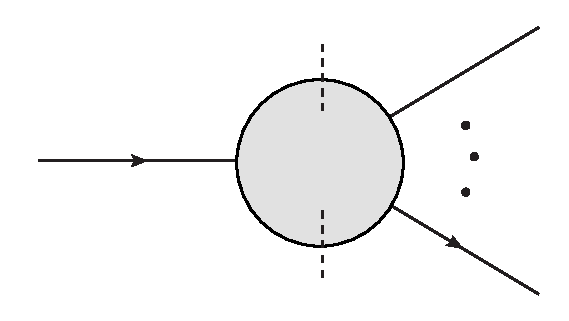
\includegraphics[height=12ex]{./figures/dc_div_left.eps}}} =
        \vcenter{\hbox{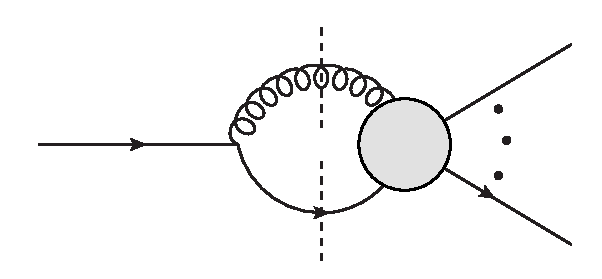
\includegraphics[height=12ex]{./figures/dc_div_r.eps}}}~+~
        \vcenter{\hbox{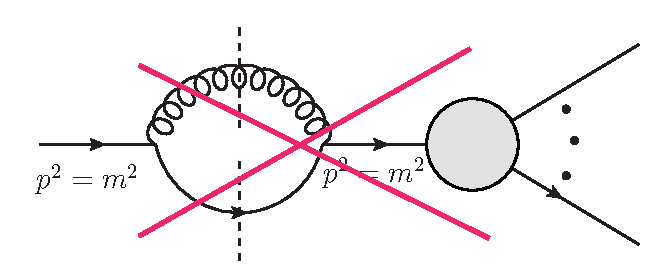
\includegraphics[height=12ex]{./figures/dc_div2_cross.eps}}}
      \]
      \caption{
        A double cut with the single on-shell massive quark in the corner (on the left), containing
        a divergent contribution associated to the mass and wave-function renormalization (the second term on the right),
        which has to be manually removed.
      }
      \label{fig:wbb:singdoublecut}
    \end{figure}
    Following the approach of \cite{Ellis:2008ir} we have implemented the removal of this contributions in our off-shell recursion.

  \item The topology in \cref{fig:dc_div2}, in addition to containing a divergent contribution mentioned above,
    has another special feature: the transverse complement of its single light-like external momentum contains this momentum.
    We discussed this in \cref{sec:ms_examples}.
    \begin{figure}[h]
      \centering
      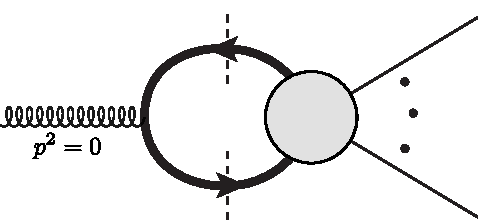
\includegraphics[width=0.3\textwidth]{dc_div2}
      \caption{A special one-loop topology with a massless on-shell leg in the corner and massive cut propagators.}
      \label{fig:dc_div2}
    \end{figure}
    This has two consequences. First, there are more coefficients with master integrals, and we evaluate the corresponding integrals explicitly.
    Second, as opposed to other one-loop topologies, the ansatz for the integrand of this topology is \emph{not} invariant under loop momentum shifts.
    This slightly complicates the construction of hierarchies, since it implies that the tadpoles below have to be carefully aligned.
    Interestingly, this is a generic feature beyond one loop, i.e.\ the ansätze for integrands of \emph{all} topologies are not invariant under loop momenta shifts.
\end{enumerate}


\paragraph{Integrals with internal masses.} Finally,
we have implemented all one-loop master integrals with real internal masses to $\order{\epsilon^0} $, based
on the results from \cite{Carrazza:2016gav,vanHameren:2010cp}. This allows us to incorporate
them in our automated numerical precision tracking and rescue system.

%%%%%%%%%%%%%%%%%%%%%%%%%%%%%%%%%%%%%%%%%%%%

\section{Setup}
\label{sec:wbb:setup}

\subsection{Channels}
\label{sec:calcsetup}

We compute NLO QCD corrections for the production of \Wbb~in association with $n$ light jets ($n =
0,1,2,3$) at the LHC $\sqrt{s} = 13$ TeV. 
We include the leptonic decays of the off-shell vector bosons at the level of amplitudes.
The parton-level cross-sections are obtained from the following channels:
\begin{subequations}
  \begin{align}
    n=0:&\qquad 0\rightarrow Wb{\bar b}q{\bar q}'\ ,\\
    n=1:&\qquad 0\rightarrow Wb{\bar b}q{\bar q}'g\ ,\\
    n=2:&\qquad 0\rightarrow Wb{\bar b}q{\bar q}'gg\ ,\quad  0\rightarrow Wb{\bar b}q{\bar q}'Q{\bar Q}\ ,\\
    n=3:&\qquad 0\rightarrow Wb{\bar b}q{\bar q}'ggg\ ,\quad  0\rightarrow Wb{\bar b}q{\bar q}'Q{\bar Q}g\ ,
  \end{align}
\end{subequations}
which we wrote in a crossing-symmetric form. 
Here the light quarks are denoted with $q$ and $Q$, and the $b$ quarks are considered massive.
The contributions from closed $b$ and $t$ loops are included. \footnote{
  Although the contribution of the latter is negligible.
}
We demonstrate some representative Feynman diagrams contributing to the channels of \Wbbjjj{} in \cref{fig:FDsWbb3j}.

We consider fixed order predictions at parton-level and discard parton-shower
effects. We will require exactly two tagged infrared-safe $b$ jets \cite{Banfi:2006hf}
in all observables we examine.

\begin{figure}[h]
  \centering
  \subfloat[][$qg\rightarrow q^\prime g g W^{\pm}b\bar{b}$]{ 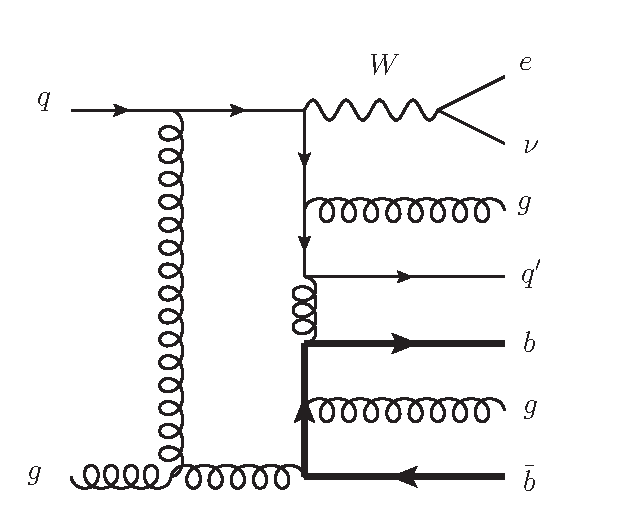
\includegraphics[width=0.28\textwidth]{figures/Wbb2q3g}}
  \qquad
  \subfloat[][$qg\rightarrow q^\prime g g W^{\pm}b\bar{b}$]{\label{subfloat:nf} 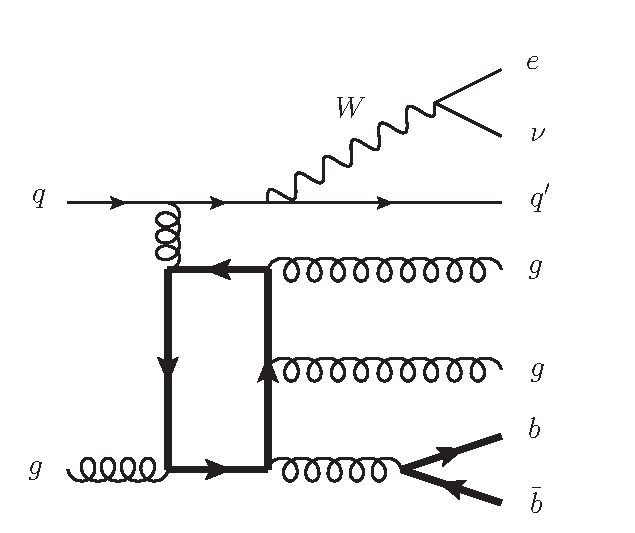
\includegraphics[width=0.28\textwidth]{figures/Wbb2q3g_nf}}
  \quad
  \subfloat[][$q{\bar Q}\rightarrow q^\prime \bar{Q} g W^{\pm}b\bar{b}$]{ 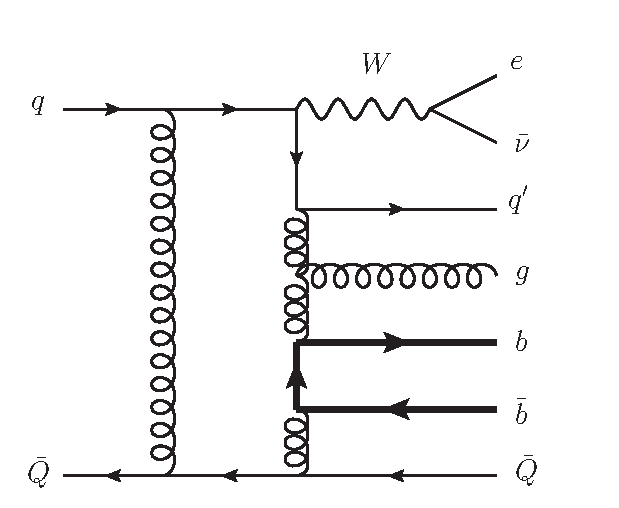
\includegraphics[width=0.28\textwidth]{figures/Wbb4q1g}}
  \caption{Representative one-loop diagrams contributing
    to \mbox{$pp\rightarrow$ \Wbbnj[3]{}} production. Massive quark
    lines are printed thick and the diagram \protect\subref{subfloat:nf} displays a contribution from closed loops of top and bottom quarks.}
  \label{fig:FDsWbb3j}
\end{figure}



\subsection{Renormalization}

We regularize UV and IR divergences in the FDH scheme in the computation of virtual matrix elements,
and use the known transition rules to convert our results to the HV scheme.

\todo{fix error in renormalization}

We give all counter-terms required for the renormalization in the FDH scheme, as well as additional finite shifts in \cref{tab:renorm}.
For the mass and wave-function renormalization we use the on-shell scheme,
and for the $\overline{\text{MS}}$ scheme for the QCD coupling.
\begin{table}[h]
  \begin{tabular}{lcll}
    \textbf{Renormalization} & \textbf{Scheme} & \textbf{Counterterm} \\
    \toprule
    Heavy quark wave function   & on-shell & $\displaystyle \delta_{2,i} ~=~ \frac{N_c^2-1}{2N_c} \left( \frac{3}{\epsilon} + 5 + 3 \ln{\frac{\mu^2}{m_i^2}} \right)$\\
    Light quark wave function   & on-shell & 0\qquad(UV+IR cancellation) \\
    Quark mass            & on-shell & $\displaystyle \delta_{m_i} ~=~ \delta_{2,i}\quad\text{}$\\
    Gluon wave function   & on-shell & $\displaystyle \delta_3 ~=~ \frac{3}{\epsilon} + \sum_i \frac{1}{3}\ln{\frac{\mu^2}{m_i^2}}$\\
    QCD coupling & $\overline{MS}$ & $\displaystyle \delta_{\alps} ~=~ \frac{1}{\epsilon} \left( \frac{11}{3}N_c - \frac{2}{3}(N_f+N_h) \right) - \frac{N_c}{3}$\\
    \midrule
    Decoupling shift & --- & $\displaystyle     \Delta_i ~=~  -\frac{2}{3}\ln{\frac{\mu^2}{m_i^2}} $\\
    \bottomrule
  \end{tabular}
  \caption{The renormalization counter-terms. Here $\mu$ is the renormalization
    scale, $m_{i}$ are the masses for heavy quarks, $N_f$ is the number of light flavors,
    $N_h$ the number of heavy flavors, and $N_c$ the number of colors.
  }
  \label{tab:renorm}
\end{table}
We set $N_f=4$, and $N_h=2$, as we work in the 4FNS, and 
add the decoupling shifts for top and bottom quarks to correctly reproduce the corresponding decoupling limits.
Except for the mass renormalization, which we perform via an explicit computation,
the whole renormalization is proportional to the tree amplitude, 
and the renormalized amplitude $\mathcal{A}^{(ren)}$ is
obtained as
\begin{equation}
  \mathcal{A}^{(ren)} =
  \mathcal{A}^{(bare)}_{m_R} - 4\pi \alpha_s c_\Gamma 
  \left( \sum_i N_{Q_i} \frac{\delta_{2,i}}{2} + N_{g}\delta_3 + \frac{N_{\alps}}{2}\left(\delta_{\alps} + \sum_{i\in N_h}\Delta_i\right) \right)  \mathcal{A}^{(born)},
  \label{renfull}
\end{equation}
where $\mathcal{A}^{(bare)}_{m_R}$ is the amplitude with renormalized masses,
$\displaystyle c_\Gamma={(4\pi)^{-(2-\epsilon)}{\Gamma(1+\epsilon)\Gamma^2(1-\epsilon)}/\Gamma(1-2\epsilon)}$,
$N_g$ and $N_{Q_i}$ are the numbers of external gluons and heavy quarks of flavor $i$ correspondingly,
and $N_{\alps}$ is the power of $\alps$ of the tree amplitude.
We shift \cite{Signer:2008va} the amplitude by
\begin{equation}
  \mathcal{A}^{(ren)}_{HV} - \mathcal{A}^{(ren)}_{FDH} = -4\pi \alpha_s c_\Gamma\left(N_{g}~\frac{N_c}{6} + \frac{N_q}{4}\left(N_c -\frac{1}{N_c}\right)\right)\mathcal{A}^{(born)},
  \label{schemeshift}
\end{equation}
to convert it to the HV scheme.



\subsection{Validation}

The upgrade to the new version of \BlackHat{} involved significant new developments,
as well as replacing a considerable number of old components.
We have extensively validated the new version with the following checks:
\begin{enumerate}
  \item We have reproduced all amplitudes available in \BlackHat{} before the upgrade.
  \item We perform a number of automated internal consistency checks:
    \begin{itemize}
      \item We extend the ansatz for the integrands on the right-hand side of \cref{eq:cut_equations} with the terms which are guaranteed to be zero, for example, by the power-counting constraints.
        We then solve the equations for the coefficients, and check if the coefficients of these term vanish.
      \item We check the known pole structure \cite{Catani:2000ef} of each primitive amplitude.
    \end{itemize}
  \item We have checked the IR poles of squared matrix elements against the integrated subtraction terms,
    as implemented in the \SHERPA{} library.
  \item We have reproduced the helicity amplitudes from \cite{Ellis:2008ir}.
  \item We have performed a systematic comparison of squared matrix elements 
    of all subprocesses of $pp\rightarrow t\bar t+(\leq 2)-$jet, $pp\rightarrow b\bar b+(\leq 2)-$, and
$Wb\bar b+(\leq3)-$ processes against publicly available generators 
\textsc{Recola}~\cite{Actis:2016mpe} and \textsc{OpenLoops}~\cite{Cascioli:2011va} 
(both powered by the \textsc{Collier} library~\cite{Denner:2016kdg}).
\end{enumerate}

\subsection{Numerical Stability}
%
In this section, we explore the numerical stability of the new version of \BlackHat{}.
We compare the normal matrix elements $d\sigma_V^\mathrm{prod}$ with the ones obtained from quadruple-precision evaluations $d\sigma_V^\mathrm{HP}$.\footnote{
  We use the \cite{QD} library for high-precision arithmetics
}

\begin{figure}[h]
  \centering
  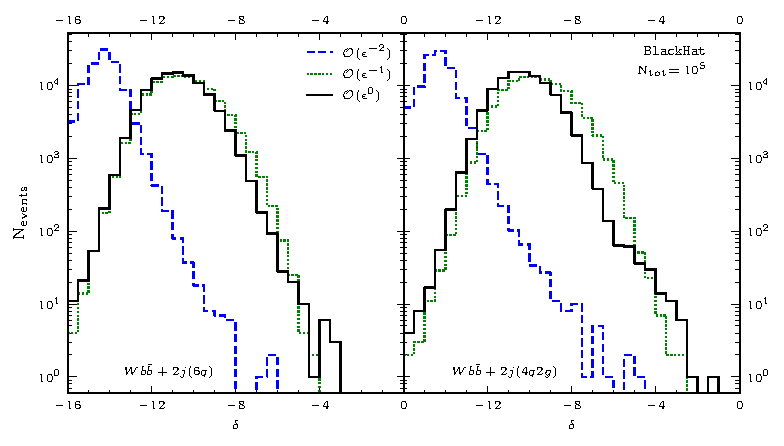
\includegraphics[scale=1.1]{plots/numstab2j}
  \caption{
    The logarithmic relative error of the full-color matrix elements
    for two types of subprocesses contributing to the \Wbbjj~production calculation. On the
    left we show results for the
    six-quark and on the right for four-quark matrix elements, respectively.
    The dashed (blue) line represents the precision of the double pole, the dotted
    (green) line represents the single pole and the
  solid (black) line the precision of the finite piece of the calculation.}
  \label{fig:stabilityWbb2j}
\end{figure}
\begin{figure}[h]
  \centering
  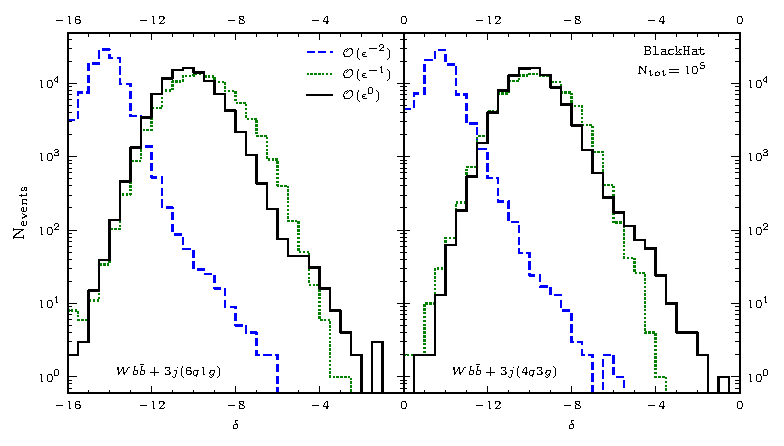
\includegraphics[scale=1.1]{plots/numstab3j}
  \caption{As in \cref{fig:stabilityWbb2j} but for \Wbbjjj{} production,
  considering only the leading-color contributions to the one-loop matrix elements.
  On the left we show results associated to the six-quark and on the right the ones associated to
four-quark matrix elements.}
\label{fig:stabilityWbb3j}
\end{figure}


We study the most complex sub-processes
by generating the histograms (see \cref{fig:stabilityWbb2j,fig:stabilityWbb3j}) of the logarithmic relative error $\delta$,
\begin{equation}
  \delta = \log_{10}\left(\frac{\left|d\sigma^{\text{prod}}_V - d\sigma^{\text{HP}}_V\right|}{\left|d\sigma^{\text{HP}}_V\right|}\right)\ .
  \label{reldiff}
\end{equation}
We sample $10^5$ phase-space points from the same distribution that we used in our phenomenological studies.
Overall we see, that our program is numerically stable,
with only a few points with precision worse then $10^{-3}$,
which have no effect on the observables.

One of the advantages of unitarity methods is that they allow a fine-grained control of the evaluation process.
We convert all the internal consistency tests listed in the previous section into
the precision-monitoring system.  
It identifies when the computation becomes unstable, and reevaluates
only the small part with higher precision whenever required.



\section{Monte Carlo Integration}
\label{sec:wbb:mc_integration}



We employ \SHERPA{}\cite{Sherpa} for managing the Monte-Carlo integration,
subprocess generation and phase-space mappings.
And we interface it to our library for virtual matrix-element generation.
We split the virtual matrix elements into leading and subleading color contributions
to optimize the integration. The latter are more expensive to compute, but contribute less to the observables,
so they can be samples less frequently \cite{BH:W3jDistributions,Ita:2011ar}.
We employ massive dipoles \cite{Catani2002} for IR subtraction as implemented in \COMIX{}~\cite{Comix}.
%

We perform a fixed-order parton-level computation. Non-perturbative effects, such as hadronization, as well as parton showers are considered in our study.
All results that we provide are fixed-order parton-level predictions and we include neither parton-shower effects nor hadronization corrections or other
non-perturbative effects.

\subsection{Input Parameters}
\label{sec:base_setup}
We use PDFs from {\texttt CT14}~\cite{CT14},
with LO ({\texttt CT14llo\_NF4}) and NLO ({\texttt CT14nlo\_NF4}) PDF sets, as
implemented in the LHAPDF library~\cite{LHAPDF}. 
The strong coupling is taken to by $\alps(M_Z)=0.125$ at LO and
$\alps(M_Z)=0.1128$ at NLO. 
The bottom-quark mass is $m_b=4.75$ GeV.

The electroweak parameters are evaluated in the LO $G_\mu$ scheme \cite{Denner2000c}. The fixed and computed
parameters as given in \cref{tab:ewinput}. The $\alpf(M_Z)$,
$\sin^2(\theta_W)$ and $g_W^2$ are computed with
\begin{align}\label{eq:ewlorel}
\sin^2(\theta_W) &= \left(1-\frac{M_W^2}{M_Z^2}\right)\ , & \alpf(M_Z)&=\frac{\sqrt{2}}{\pi}G_F M_W^2
  \sin^2(\theta_W)\ ,\notag\\
g_W^2&=\frac{4\pi\alpf(M_Z) }{\sin^2(\theta_W)}\ .
\end{align}

\begin{table}[]
  \centering
  \begin{tabular}{p{3.5cm}p{5cm}}
    \toprule
    Parameter & Value  \\
    \midrule
    $G_F$ & $1.1663787 \times 10^{-5}$ GeV$^{-2}$ \\
    $M_W^{\text{OS}}$& $80.385$ GeV \\
    $M_Z^{\text{OS}}$& $91.1876$ GeV \\
    $\Gamma_W$& $2.085$ GeV \\
    $\alpf(M_Z)$ & $1/132.23$ (calculated)\\
    $\sin^2(\theta_W)$ & $0.22290$ (calculated)\\
    $g_W^2$ & $0.42635$ (calculated)\\
    \bottomrule
  \end{tabular}
  \caption{Electroweak parameters used in our study, which are chosen in accordance with 2016 PDG values~\cite{Patrignani:2016xqp}.}
  \label{tab:ewinput}
\end{table}

The CKM matrix is approximated by a unit matrix. 
The leads to difference of  the order of at most 1\%,
as determined from the LO analysis.

We find that the contribution of the closed top quarks has a order $1\%$ effect on
the cross-sections. This is according to expectations ~\cite{BH:W4j,BH:Z4j,Campbell:2016tcu}. 

\subsection{Kinematics and Observables}
\label{sec:kin}
In this section, we provide the definition for observables we employ in our study.
The pseudorapidity $\eta$ and the
angular separation between two partons, leptons, or jets $\Delta R$ are defined as
\begin{align}
  \eta &= -\ln\left(\tan\frac{\theta}{2}\right),&  \Delta R &= \sqrt{(\Delta \phi)^2+(\Delta \eta)^2}.
\end{align}
Here $\Delta\phi$ is the difference in the azimuthal angle in the transverse plane,
$\theta$ is the polar angle with respect to the beam axis, and
$\Delta\eta$ the difference in $\eta$. 
The transverse energy of $W$, $E_T^W$, and the total partonic transverse energy $\HTpartonicp$ are defined as
\begin{align}\label{eq:htpart}
  E_T^W&=\sqrt{M_W^2+\left(p_T^W \right)^2},& \HTpartonicp&=\sum_j p_{\textrm T}^j+E_{\textrm T}^W, \qquad p_T=\sqrt{p_x^2+p_y^2}
\end{align}
with the sum over all final state partons $j$.
The jet invariant masses are defined by
\begin{align}
  M_{ij}^2 = \left(p_i^{\text{jet}}+p_j^{\text{jet}}\right)^2,
\end{align}
and we label  jets in order of decreasing transverse momentum $p_T$. 
The transverse mass of $W$ is
\begin{align}
  M_T^W=\sqrt{2E_T^eE_T^\nu(1-\cos(\Delta\phi_{e\nu}))}\ .
\end{align}

We now explain how do we build the exclusive-sum observables from multi-jet samples.
We choose the cut $p_{T}^{\text{excl}}$, with respect to which we take an exclusive cross-section $\sigma^{\text{exc}}_n$
for each jet multiplicity $n$, except the one with maximal  $n$, for which we take the inclusive result,
\begin{align}\label{eq:excsums}
  \sigma^{\text{NLO+}}_0 &= \sigma^{\text{exc}}_0 + \sigma^{\text{inc}}_1\ , &
\sigma^{\text{NLO++}}_0 &= \sigma^{\text{exc}}_0 +\sigma^{\text{exc}}_1+
\sigma^{\text{inc}}_2\ .
\end{align}
The expectation is that replacing the, effectively leading order contributions, from the real radiation with the full NLO
corrections mitigates the problem of large $K$ factors, and at the time, the sensitivity to $p_{T}^{\text{excl}}$ is not as high 
as in the case of the exclusive computation.

\section{Phenomenology}
\label{sec:wbb:pheno}
In this section we present our predictions for the \Wbbn~production in
$pp$ collisions in NLO QCD precision at $\sqrt{s}=13$ TeV. 
We apply the following cuts
\begin{align}
  p_T^{\text{jet}}&>25\text{ GeV},& |\eta^{\text{jet}}|&<2.4\ ,\notag\\
  p_T^{e}&>25\text{ GeV},& |\eta^{e}|&<2.5\ ,\notag\\
  p_T^{\nu}&>20\text{ GeV},& M_T^W &> 20\text{ GeV}\ .
  \label{eq:Cuts}
\end{align}
to all jets (including $b$ jets).
We employ the standard dynamical choice of factorization and renormalization scales $\mu_R=\mu_F=\mu_0=\HTpartonicp/2$ (see \cref{eq:htpart}).
We estimate the error from the missing orders of the perturbation series expansion in the coupling constants with the standard technique of
the scale variations around the central scale $\mu_0$. 
We define jets with the anti-$k_T$ jet algorithm~\cite{antikT} with $R=0.4$, as implemented in the
\texttt{FastJet} package~\cite{Cacciari:2011ma}.

\subsection{Total Cross Section and Scale Dependence}
\label{totalxsw}
First, we show our results for fiducial partonic cross sections (defined by the cuts \cref{eq:Cuts})
for the inclusive production of $W^{\pm}b\bar{b}$ for all considered jet multiplicities in \cref{tab_Wpj_total_xs}.
And we display their scale-dependence in \cref{fig_Wjets_sdep}.

We observe, as expected, that the LO cross-sections are very sensitive to the scale variations,
except for the case of \Wbb{} cross-section.
The latter is not representative of the errors of the LO result, due
to the large $K$-factor from the opening of the gluon-initiated channel~\cite{Ellis:1998fv,FebresCordero:2006sj,Cordero:2009kv},
as well the kinematical constraints for $p_T^{b\bar b}$ and $p_T^W$.
For \Wbbj{}, also the channel with two gluons in the initial state is opened.
Starting from two additional light jets, all subprocesses contribute already at LO,
and we observe a better-controlled perturbative series expansion.
It is then expected, that with even larger number of light jets,
the jet-universality is reached \cite{BH:Wratios,BH:W5j}.


%%%%%%%%%%%%%%%%%%%%%%%%%%%%%%%%%%%%%%%%%%%%%% 
\begin{table}[ht]
  \begin{center}
    \begin{adjustbox}{width=1\linewidth}
      \begin{tabular}{ccccccc}
        \toprule
        jets  & \Wbbm~LO & \Wbbm~NLO & $K$-factor & \Wbbp~LO & \Wbbp~NLO & $K$-factor\\
        \midrule
        0  & $0.33278(12)^{+0.0619}_{-0.0490}$ & $0.67719(60)^{+0.1288}_{-0.1000}$  & $2.03$ & $0.48573(19)^{+0.0925}_{-0.0727}$ & $0.97175(85)^{+0.1877}_{-0.1411}$  & $2.00$\\
        1  & $0.36153(13)^{+0.1408}_{-0.0945}$ & $0.50484(63)^{+0.0851}_{-0.0800}$  & $1.40$ & $0.52095(23)^{+0.2034}_{-0.1362}$ & $0.72740(99)^{+0.1277}_{-0.1167}$  & $1.40$\\
        2 & $0.18501(44)^{+0.1053}_{-0.0626}$ & $0.22604(87)^{+0.0407}_{-0.0400}$  & $1.22$ & $0.27663(68)^{+0.1569}_{-0.0934}$ & $0.3340(17)^{+0.0599}_{-0.0647}$  & $1.21$\\
        3  & $0.07204(25)^{+0.0540}_{-0.0289}$ & $0.08288(89)^{+0.0189}_{-0.0200}$  & $1.15$ & $0.11493(59)^{+0.0855}_{-0.0459}$ & $0.1286(17)^{+0.0280}_{-0.0307}$  & $1.12$\\
        \bottomrule
      \end{tabular}
    \end{adjustbox}
     %%%%%%%%%%% TABLE xs  %%%%%%%%%%%%%%%%%%%%%%%%%%
  \end{center}
  \caption{LO and NLO QCD results for inclusive \Wbbpm+$0,1,2,3$-jet cross
    sections (in $pb$). Results with dynamical scale $\HTpartonicp/2$ are shown
    together with their respective $K$-factors.  The setup employed is specified in
    section~\ref{sec:kin}, and kinematical cuts in \cref{eq:Cuts}. Scale
    dependence is shown in superscripts and subscripts. The number in parenthesis next to
    the central value gives the corresponding statistical integration
    error.\label{tab_Wpj_total_xs} }
  \end{table}


%scale dependence for Wm
%%%%%%%%%%%%% FIGURE %%%%%%%%%%%%%%%%%%
\begin{figure}[t]
\begin{center}
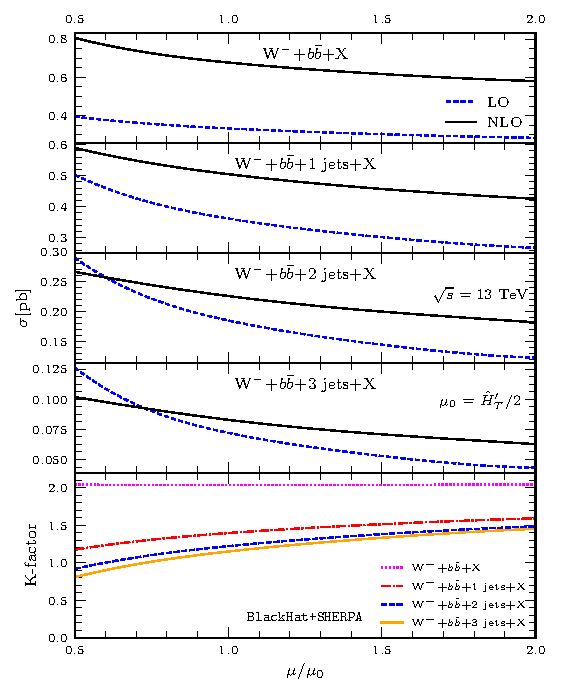
\includegraphics[clip,scale=0.71]{plots/scale_dependence_Wmbb}
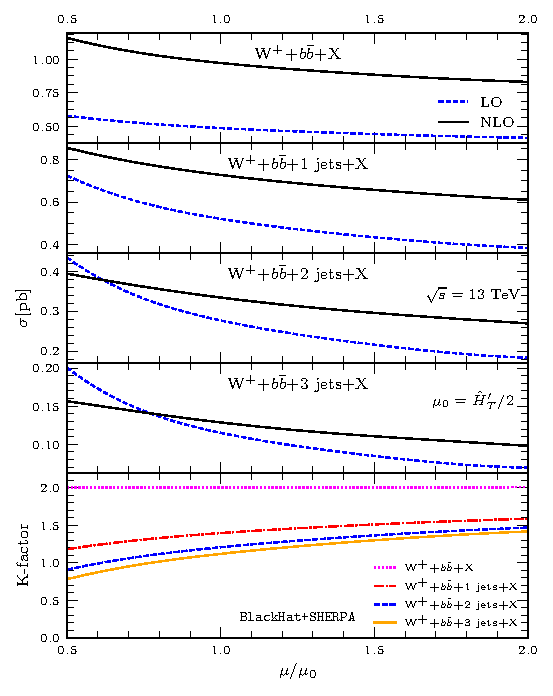
\includegraphics[clip,scale=0.71]{plots/scale_dependence_Wpbb}
\end{center}
\caption{The renormalization- and factorization-scale dependence of total cross
  sections for \Wbbm$+0,1,2,3$-jet$+X$ production in the left and
\Wbbp$+0,1,2,3$-jet$+X$ production to the right,
 with $\mu_0=\mu_\mathrm{r}=\mu_\mathrm{f}=\HTpartonicp/2$. 
The upper four panels show the dependence of LO (dashed blue line) and
  NLO (solid black line) predictions. The lower panel shows
  the K-factor (ratio of NLO/LO).}
\label{fig_Wjets_sdep}
\end{figure}
%%%%%%%%%%%%%%%%%%%%%%%%%%%%%%%%%%%%%%%

It is interesting to compare these results with the similar studies of the $W^{\pm}$ production in association with light jets only \cite{BH:W3jPRL,BH:W4j,BH:W5j,Mangano:2016jyj}.

First of all, we notice that the central value for the NLO cross-section consistently tends towards the right end of the plateu,
which was not the case in the light-jet-only studies. We attribute this
to the different types of dominant subprocesses\footnote{and \emph{not} to the mass effects}.
In our case, these are the ones with two quark lines.
And in the light-jet production, these are the ones with a single quark line.

Second, although we do not show it on the plots,
the subleading-color contributions are more important in the case of \Wbbn{} production,
and are of the order of $10\%$, as opposed to  $\lesssim 3\%$ for the $W$+jets production.
This is caused by the fact, that the contribution of the virtual part
is dominating the total cross-section in our case.

\subsection{Differential distributions}
\label{diffxsw}

In this section, we show our prediction for a number of differential distributions.

%pt leading bjet
%%%%%%%%%%%%% FIGURE %%%%%%%%%%%%%%%%%%
\begin{figure}[ht]
  \centering
  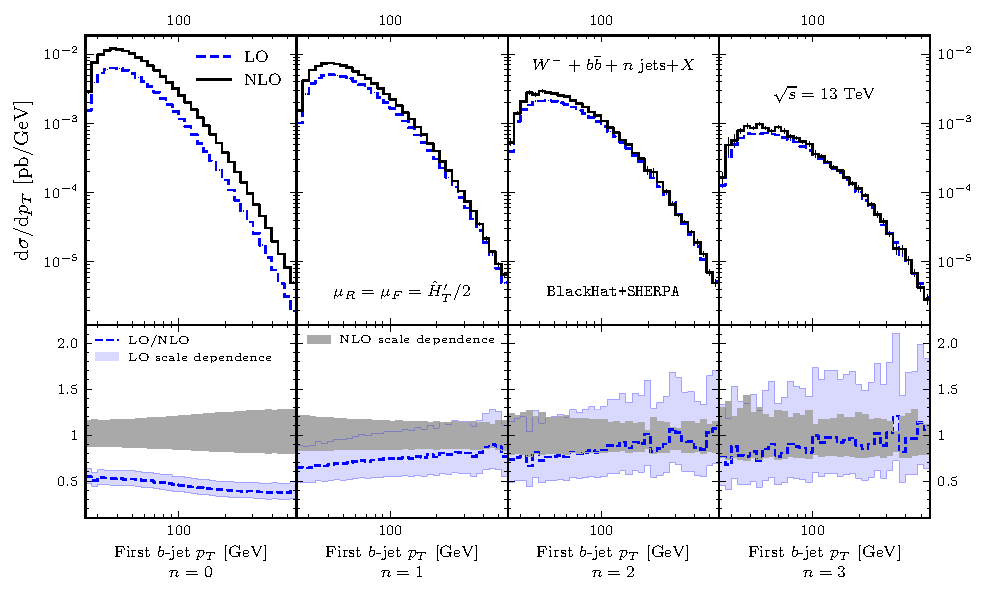
\includegraphics[clip,scale=1]{plots/ptleading}
  \caption{The $\pT$ distributions of the leading $b$ jet (ordered by $p_T$) in inclusive \Wbbm$+n$-jet
    production at the LHC with $\sqrt{s}=13$~TeV. The light-jet multiplicity 
    increases from $n=0$ to $n=3$ from left to right. In the upper panels the
    dashed (blue) lines show the LO results and the solid (black) lines the NLO
    results. Vertical thin lines show the statistical error from the numerical
    integration. In the bottom panels we show the scale-dependence bands
  normalized to the NLO result, in blue for LO and dark gray for NLO.}
  \label{fig_Wmnjpt}
\end{figure}
%%%%%%%%%%%%%%%%%%%%%%%%%%%%%%%%%%%%%%%

%pt subleading bjet
%%%%%%%%%%%%% FIGURE %%%%%%%%%%%%%%%%%%
\begin{figure}[ht]
  \centering
  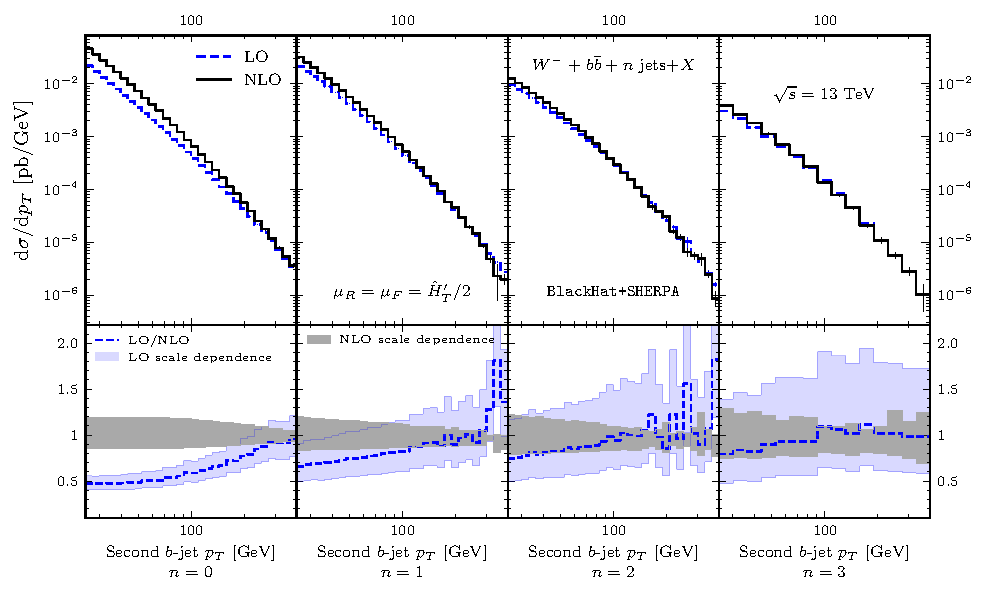
\includegraphics[clip,scale=1]{plots/ptsubleading}
  \caption{The $\pT$ distributions of the subleading $b$ jet (ordered by $p_T$) in inclusive \Wbbm$+n$-jet
    production at the LHC with $\sqrt{s}=13$~TeV. Format as in \cref{fig_Wmnjpt}.}
    \label{fig_Wmnjpt2}
  \end{figure}
%%%%%%%%%%%%%%%%%%%%%%%%%%%%%%%%%%%%%%%

In \cref{fig_Wmnjpt,fig_Wmnjpt2} we demonstrate the jet-$p_T$ distribution of the leading
and subleading $b$ jets (ordered by $p_T$) respectively. 
We observe some interesting differences in the shapes of the $p_T$ distributions between
LO and NLO, which fade out with the increasing light just multiplicity.
This feature shows up in most of the observables, and is in agreement to our arguments in the previous section.
We also note, that for high light-jet multiplicity  the NLO results lie inside the LO bands,
which is a signature of perturbative convergence.

%HT jet / hadronic
%%%%%%%%%%%%% FIGURE %%%%%%%%%%%%%%%%%%
\begin{figure}[ht]
  \centering
  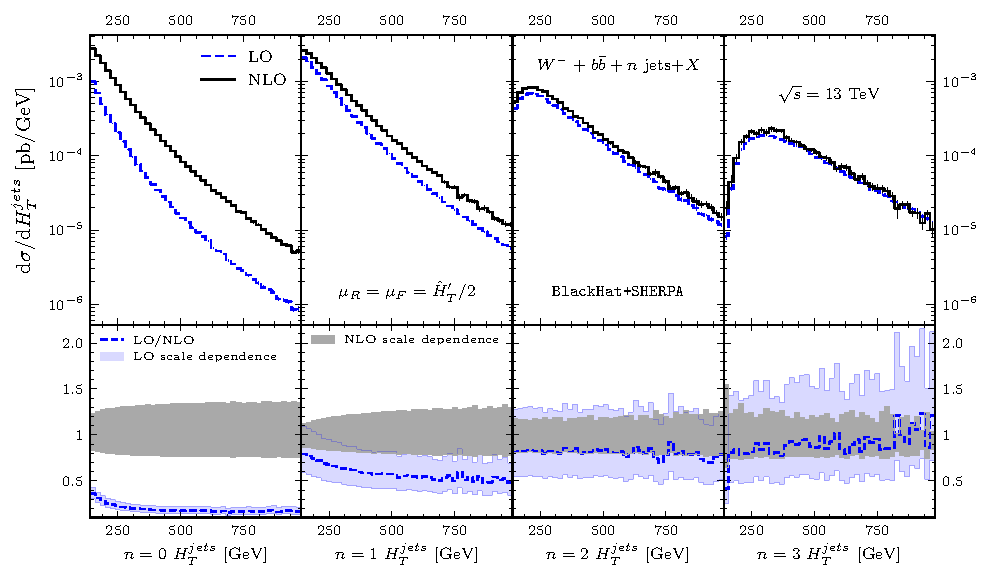
\includegraphics[clip,scale=1.0]{plots/htjets.pdf}
  \caption{Distribution in the total transverse jet energy
    $H_T^{jets}$ of light  and $b$ jets for inclusive \Wbbm$+n$-jet
    production at the LHC with $\sqrt{s}=13$~TeV. Format as in \cref{fig_Wmnjpt}.}
    \label{fig_Wmnjht}
  \end{figure}
%%%%%%%%%%%%%%%%%%%%%%%%%%%%%%%%%%%%%%%

The next observable we explore in \cref{fig_Wmnjht} is the total hadronic activity in the detector,
which in particular relevant for beyond-the-standard-model searches.
Here a new feature is that the large quantum corrections, reaching a factor of two, are observed not only for the \Wbb{}, but also for the  \Wbbj{} production. 

%dR first b-jet / charged lepton
%%%%%%%%%%%%% FIGURE %%%%%%%%%%%%%%%%%%
\begin{figure}[ht]
  \centering
  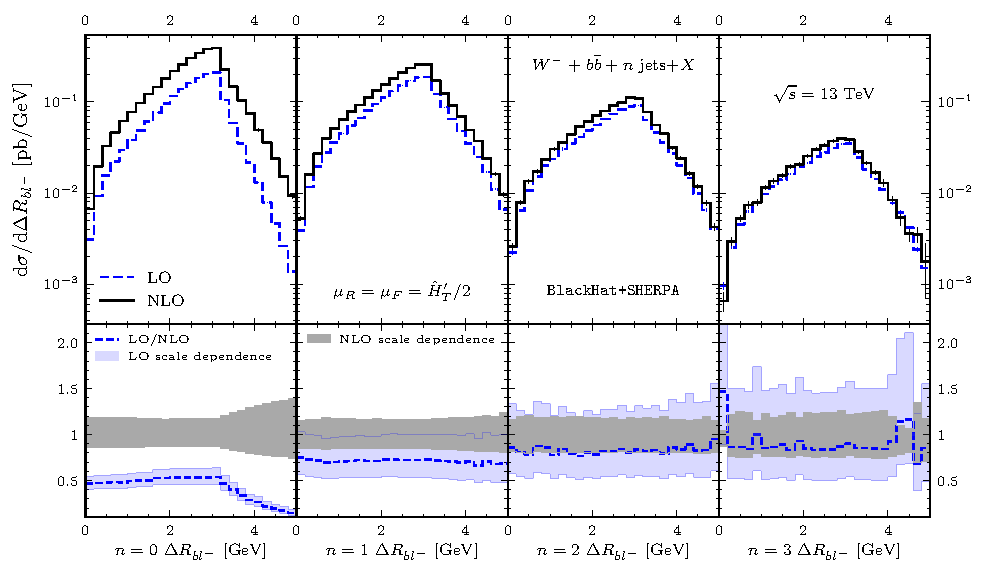
\includegraphics[clip,scale=1.0]{plots/drbl.pdf}
  \caption{Distribution in the $\Delta R_{bl^-}$ separation between the first
  $b$ jet (ordered in $p_T$) and the charged lepton for inclusive \Wbbm$+n$ jets
  production.  Format as in \cref{fig_Wmnjpt}.}
  \label{fig_Wmnjdrbl}
\end{figure}
%%%%%%%%%%%%%%%%%%%%%%%%%%%%%%%%%%%%%%%

Finally, we present in \cref{fig_Wmnjdrbl} the distribution of the angular separation  $\Delta R$ between the first $b$ jet and charged lepton $l^-$.
For this observable the NLO corrections do not introduce any significant effects, except for the case of \Wbb{} production.
In this case, the $b$-jet system and the $W$ boson are produced back-to-back, and the $\Delta \eta$ distribution peaks at zero,
hence the sharply decaying distribution at LO.
For higher light jet multiplicities these constraints are lifted.


\subsection{Finite $b$ Mass Effects}
\label{sec:bmass}


In this section, we study the effects of the finite $b$-quark mass on the observables.
We perform an analysis of the $M_{b\bar{b}}$ distribution in \Wbbnj[1]{} production,
obtained in two schemes, which treat the $b$ quark differently. 
In the 4FNS the $b$-quark mass is consistently included. 
And in the 5FNS the bottom quark is added to the list of light flavors.%
\footnote{For this scheme we use PDFs from CT14~\cite{CT14}}.
We show the ration of these two computations in \cref{fig:ratWmmbb}.


As has been argued in the previous similar studies \cite{FebresCordero:2006sj},
the effects are expected to be small, if the two $b$-jets are well separated,
and the value of $m_b^2$ is negligible compared to the relevant invariants.
This is indeed what we observe in \cref{fig:ratWmmbb}.
We have strong deviation between the two computations in the region where the ration $m_b^2/M_{b\bar{b}}^2$ 
is less or equal 1. And in the region $m_b^2/M_{b\bar{b}}^2\gg 1$ the two computations tend to the agreement.
Furthermore, we observe the stability of mass effects with respect to quantum corrections. 


%mbb spectrum Wbb & Wbbj ratio massive/massless
%%%%%%%%%%%%% FIGURE %%%%%%%%%%%%%%%%%%
\begin{figure}[ht]
  \centering
  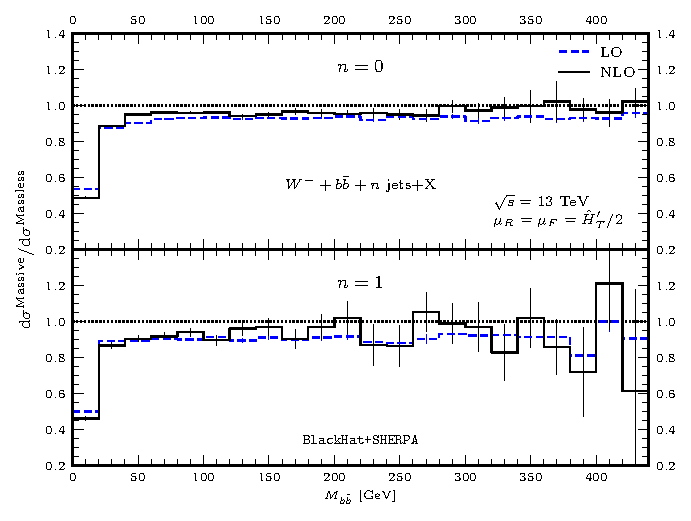
\includegraphics[clip,scale=1.0]{plots/crmbb}
  \caption{Ratio of the invariant mass spectrum of the $b\bar b$ system for 4FNS
    result to the 5FNS ones, for \Wbbm{} (top) and \Wbbm+1-jet (bottom) production.
    The ratios are taken at LO (dashed blue line) and at NLO (solid black line).
    Statistical errors are shown as thin vertical lines. We include a dotted
  horizontal line at a ratio value of 1.}
  \label{fig:ratWmmbb}
\end{figure}
%%%%%%%%%%%%%%%%%%%%%%%%%%%%%%%%%%%%%%%

We point out, that our findings are very similar to the ones of \cite{FebresCordero:2006sj},
where no additional emissions of light jets were considered.
It is also worth noting, that
there are no $b$-initiated subprocesses in the calculation  of the \Wbbnj[1]{} production,
which we study here.
Therefore, we can attribute the $b$-quark-mass effects to the virtual matrix elements,
the phase-space generation, and the differences in PDFs.
In this regard, it would be interesting to also compare for the cases of \Wbbjj{} and \Wbbjjj{}
productions.

%%%%%%%%%%%%%%%%%%%%%%%%%%%%%%%%%%%%%%%%%%%%


\subsection{Backgrounds to The Associated Production of $H$ and $W$}
\label{sec:hw}

Currently, by the end of the run II of the LHC,
the measured properties of the Higgs boson are
in general agreement with the SM predictions (see e.g.\ \cite{Khachatryan:2016vau}).
The recent discovery of the Higgs boson decay to a pair of bottom quarks \cite{Sirunyan:2018kst,Aaboud:2018zhk}
further contributes to the picture, 
and it is of great importance to accurately measure the Yukawa coupling $y_b$.

The experimental measurement of the Higgs decaying into a bottom-quark pair
is very challenging due to the dominant QCD production of $b\bar{b}$-pairs.
Considering the associated production of the Higgs with a vector boson 
helps to mitigate the backgrounds, and, indeed, this is how this decay has been discovered.
Of course, the irreducible SM background to the \Wbb{} final state is still very large,
and it is crucial to have a precise theoretical understanding of this background. 
We believe, that the NLO QCD predictions we have presented in \cite{Anger:2017glm} and
in this thesis, will contribute to this goal.

One of the most important observables for the $HW$ studies are those associated to the $b\bar
b$ system: $p_T^{b\bar b}$ and $M_{b\bar b}$.
With respect to the Higgs, these observables are directly linked to its transverse momentum and the invariant mass. 
Also, the observables associated to the associated $W$-boson are of interest, such as $p_T^W$.
We study all these observables in this section, taking advantage of our light-jet-multiplicity samples.

As we mentioned earlier, the same final-state signature can
be produced from the various combinations $\alpha$ and $\alpha_s$ (see \cref{fig:wbb_channels}). 
And some of them are enhanced by the top-quark resonances at higher energies \cite{Denner:2017kzu},
but are less relevant in the context of $HW$ production.
Nevertheless, the non-resonant contributions from the other channels can be of the similar order
as the ones we present here. We leave the study of these contributions to future work.

%pt(bb) 
%%%%%%%%%%%%% FIGURE %%%%%%%%%%%%%%%%%%
\begin{figure}[ht]
  \centering
  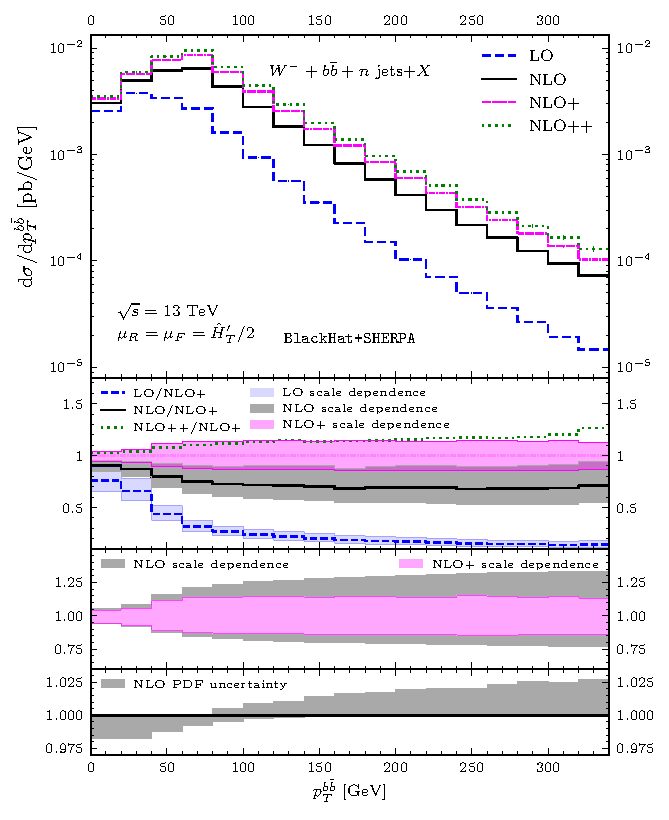
\includegraphics[clip,scale=1]{plots/excl_ptbb_v4}
  \caption{The $p_T$ distribution of the $b\bar{b}$ system in inclusive \Wbbm{} production,
    computed at LO (dashed blue line) and NLO (solid black line) as well as
    by employing the exclusive sums NLO+ (dashed-dot magenta line)
    and NLO++ (dotted green line).
    The second panel shows scale dependence bands normalized by NLO+,
    and in the third panel they are normalized by the corresponding
    central value. The bottom panel shows the associated PDF uncertainties
    normalized to our NLO results.}
  \label{fig_Wmnjptbb}
\end{figure}
%%%%%%%%%%%%%%%%%%%%%%%%%%%%%%%%%%%%%%%

As we already discussed before, the inclusive fixed-order computation
of the \Wbb{} production suffers from the large NLO QCD corrections.
And the exclusive predictions, which veto extra jets have the problem of sensitivity
to the $p_T^\mathrm{veto}$ cut~\cite{Tackmann:2012bt}. 
Here we use the exclusive-sum technique \cite{ESums}
to try to work around these problem (see the explanation in \cref{sec:kin}).
It is exactly in the case of large $K$ factors due opening of new production channels, when
the exclusive sums are expected to provide more stable predictions (see e.g.\ comparison to the data in \cite{Aad:2014qxa,ATLAS:ratio2017}). 
It is worth noting, that the addition of parton showers \cite{Luisoni:2015mpa},
or using the techniques of MEPS@NLO \cite{Hoeche:2012yf} or FxFx \cite{Frederix:2012ps}
is important for the comparison with the LHC data.


In addition to the theoretical uncertainties due to the missing higher orders, estimated
by the scale variations, we also study the PDF uncertainties, which 
they turn out to be subleading. 
We employ the error sets from \texttt{PDF4LHC15\_nlo\_nf4\_30}~\cite{Butterworth:2015oua}. 
The uncertainties associated to other sources, such as the values values of $m_b$ and $\alps$,
are expect to be subdominant.

%pt(W) 
%%%%%%%%%%%%% FIGURE %%%%%%%%%%%%%%%%%%
\begin{figure}[ht]
  \centering
  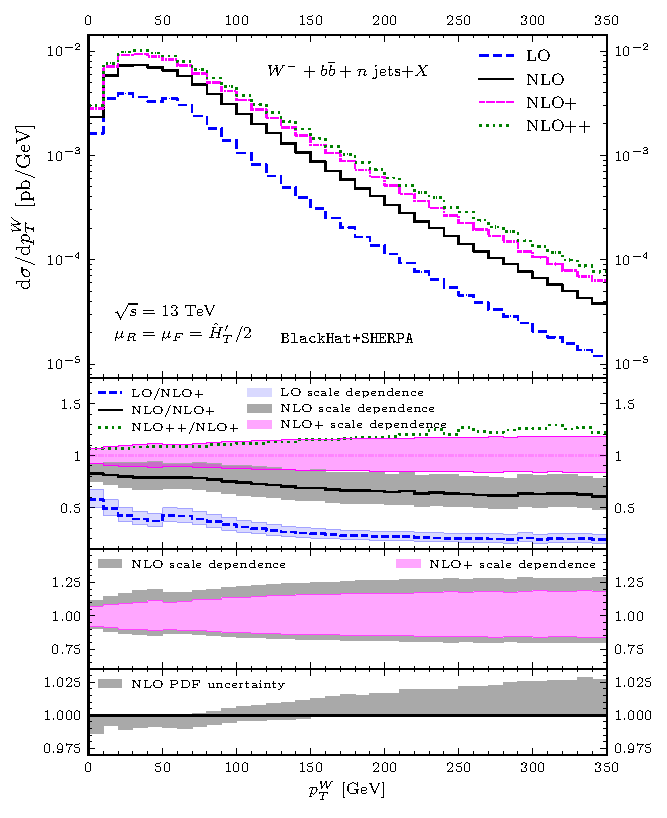
\includegraphics[clip,scale=1]{plots/excl_ptw_v4}
  \caption{The $p_T$ of the $W$ boson in inclusive \Wbbm{} production. Format as in \cref{fig_Wmnjptbb}.}
  \label{fig_Wmnjptw}
\end{figure}
%%%%%%%%%%%%%%%%%%%%%%%%%%%%%%%%%%%%%%%

First, we show our predictions  for the transverse momentum distribution of
the $b\bar b$ system in \cref{fig_Wmnjptbb}.
We show the NLO+ as well as LO, NLO and NLO++ results in the upper panel.
The former is our main prediction.
The second panel shows the corresponding scale-variation bands normalized by NLO+.
The third panel displays the comparison between the bands of NLO and NLO+, normalized by their central value.
In the bottom panel we show the PDF uncertainties. 
We observe, that the scale-dependence of the NLO+ is reduced compared to that of the NLO result,
and the corresponding bands overlap.
 
%Mbb 
%%%%%%%%%%%%% FIGURE %%%%%%%%%%%%%%%%%%
\begin{figure}[ht]
  \centering
  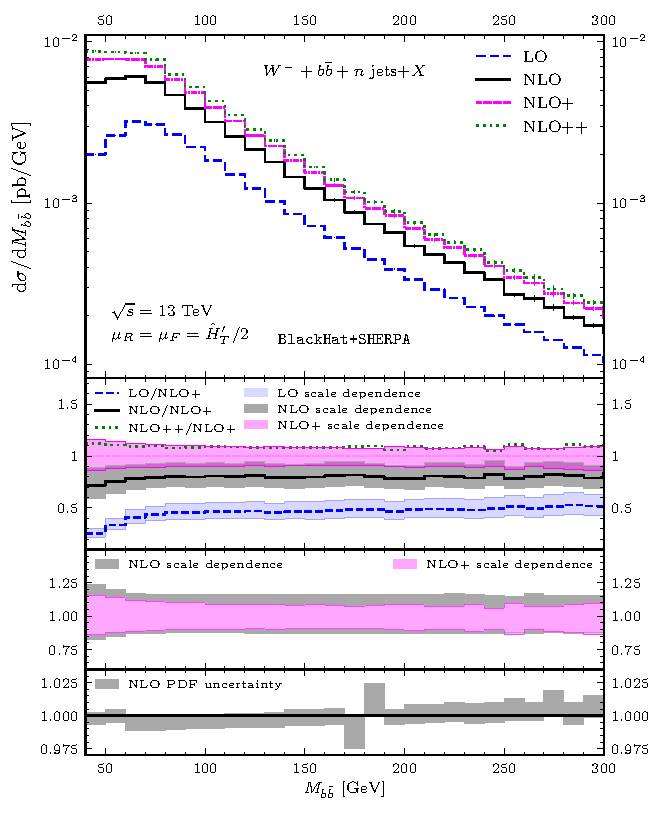
\includegraphics[clip,scale=1]{plots/excl_mbb_v4}
  \caption{The invariant mass of the $b\bar b$ system in inclusive \Wbbm{} production. Format as in \cref{fig_Wmnjptbb}.}
  \label{fig_Wmnjmbb}
\end{figure}
%%%%%%%%%%%%%%%%%%%%%%%%%%%%%%%%%%%%%%%

In \cref{fig_Wmnjptw,fig_Wmnjmbb} we show
our predictions for the transverse momentum of the $W$, and
for the invariant mass of the bottom-quark pair respectively.
The features of these predictions are similar to what we observer for
the $p_T^{b\bar{b}}$ observable, with the NLO+ uncertainty estimation marginally
overlapping with the NLO predictions.

